\documentclass[11pt,a4paper]{report}
\usepackage{amsmath,amssymb,fancyhdr,hyperref,url}
\usepackage{graphicx, geometry, layout,color}
\usepackage{fancyhdr}
\usepackage{amsthm}
\usepackage{natbib}
\usepackage{hyperref}
\usepackage{float}
\usepackage{graphicx}
\usepackage{tikz}
\usepackage{lineno}
\usepackage[toc,page]{appendix}
\usepackage{setspace}
\usepackage{caption}
\usepackage{textcomp}
\usepackage [english]{babel}
\usepackage[autostyle]{csquotes}
\usepackage{cancel}
\usepackage{lscape}
\usepackage{url}
%\MakeOuterQuote{"}

\begin{document}

\title{Sins-Lab Sputter Ion Gun Power Supply User manual}
\date{13 October 2020}
\author{edited by David McCall \\ resources provided by Dr. Sosolik \\ SINS-lab \\ Clemson University Astronomy and Physics Department}
\maketitle
\clearpage

\tableofcontents


\newpage

%the page style puts a line at the top of the page and the head puts a letter head with todays (last ran latex code) date
\pagestyle{fancy}
\lhead{\today} 

%---------------------------------------------------------------------------------------------------------------------------------------------------------------------
\chapter{Sputter Ion Gun Power Supply (SIGPS)}
%---------------------------------------------------------------------------------------------------------------------------------------------------------------------
This manual will go over the basics of plugging up the sputter power supply to the sputter gun, and running the power supply. The power supply is displayed below.

%how to do a figure
\begin{figure}[H]
\includegraphics[width=0.75\textwidth]{SIGPS.png}
\caption{This shows the sputter ion gun power supply. }
\label{SIGPSa}
\end{figure}

%======================
\section{What is the goal?}
%=====================
When one wants to clean a sample to be used in an Ulta High Vacuum (UHV) system for experiments and you want to study only the effects of the sample with the ion beam interacting with that sample, you need to get the oxide layer off of this surface. This oxide layer is usually formed by being exposed to 760 torr air molecules. In order to remove this oxide layer one sputters the surface of the sample. Sputterting is done by bombarding the sample with  ionized noble gas ions on the surface. Afterwards the surface has to be reoriented which is usually done by heating/annealing the surface at a certain temperature. In this manual we will primarily talk about the device used to sputter ionized noble gases to the sample which we call this device a sputter gun. This sputter gun and power supply was developed originally at Cornell University around the early $90's$ by Dr. Cooper's research group.   

%------------------------------------------------------------------
%----------------------------Date manual was updatedConnections----------------------------
%-------------------------------------------------------------------------------------------
\section{Info in manual}
%-------------------------------------------------------------------------------------------------------------------------------------------------------------
This information is current as of October 13th, 2020.

%--------------------------------------------------------------------------------------
\subsection{General Information}
This equipment is destined for use with a sputter gun. The user should read this instruction manual and any other additional information referred to in this manual before operating this equipment. David McCall will not be held responsible for any events occuring due to noncompliance, even partial, with these instructions, improper use by untrained persons or any action contray to that provided for by this manual. This power supply controls the power going into the sputter gun which allows sputtering on samples inside an Ultra High Vacuum chamber. This device contains high voltage parts and should be handled with care. Probing the highvoltage parts should be done with a high voltage probe and the appropriate safety equipment.



%------------------------------------------------------------------
%----------------------------Materials----------------------------
%-------------------------------------------------------------------------------------------
\subsection{Materials}
{In  order to use the sputter gun you will need:}
\begin{enumerate}
	\item  Four coaxial cables
	\item Two external high voltage power supplies
	\item  Sputter gun
           \item  Ultra High Vacuum Chamber with 
      \begin{enumerate}
                 \item pressor sensors 
                 \item  sample
                 \item device to measure the current hitting the sample
       \end{enumerate}
           \item  Digital multimeter with a high voltage probe 
\end{enumerate}


%------------------------------------------------------------------
%----------------------------Connections----------------------------
%-------------------------------------------------------------------------------------------
\subsection{Connections}
In this subsection we will break down the connections from the Sputter Ion Gun Power Supply to to the sputter gun and an external power supply in order to use the supply with the sputter gun to sputter ions onto a surface for cleaning.

%%%%%%%%%%%%%%%%%%%%%%%%%
\subsubsection{Connection output from SIGPS to Sputter gun}
%%%%%%%%%%%%%%%%%%%%%%%%%
There are three wires/BNC connectors that connect from the Sputter Ion Gun Power Supply (SIGPS) to the Sputter gun. These are the Anode, COM, and Filament connections at the top row of the SIGPS from left to right, respectively, as displayed in figure \ref{SIGPSa}. 

%%%%%%%%%%%%%%%%%%%%%%%%%%%%%%
\subsubsection{Connection from SIGPS to external power supply}
%%%%%%%%%%%%%%%%%%%%%%%%%%%%%%
There Beam voltage is outsourced from the SIGPS to an external high voltage power supply. In our test prior to using this manual we chose the Glassman High Voltage Power Supply because it was available and worked. Displayed below is the HVPS that we utilized. Make sure that your High Voltage Power Supply is grounded prior to use. We grounded it to our common ground with a ground cable connected to the bars that were used for support for our Ultra High Vacuum Chamber.
\\
The way this works is you just connect a high voltage power supply's (HVPS)  output into the beam voltage. Then make sure all of the knobs, potentiometers, are turned counterclockwise until they can't go any further. This establishes a zero voltage and current output. Next turn on the HVPS on and use the HVPS to adjust what the beam voltage would be for the SIGPS. Then press the green High Voltage button. {\bf If you don't press this button the knobs will not display current nor volts and you will not get anything out of thte power source!} Now you can adjust the voltage coming out of the external High Voltage Power Supply.


\begin{figure}[H]
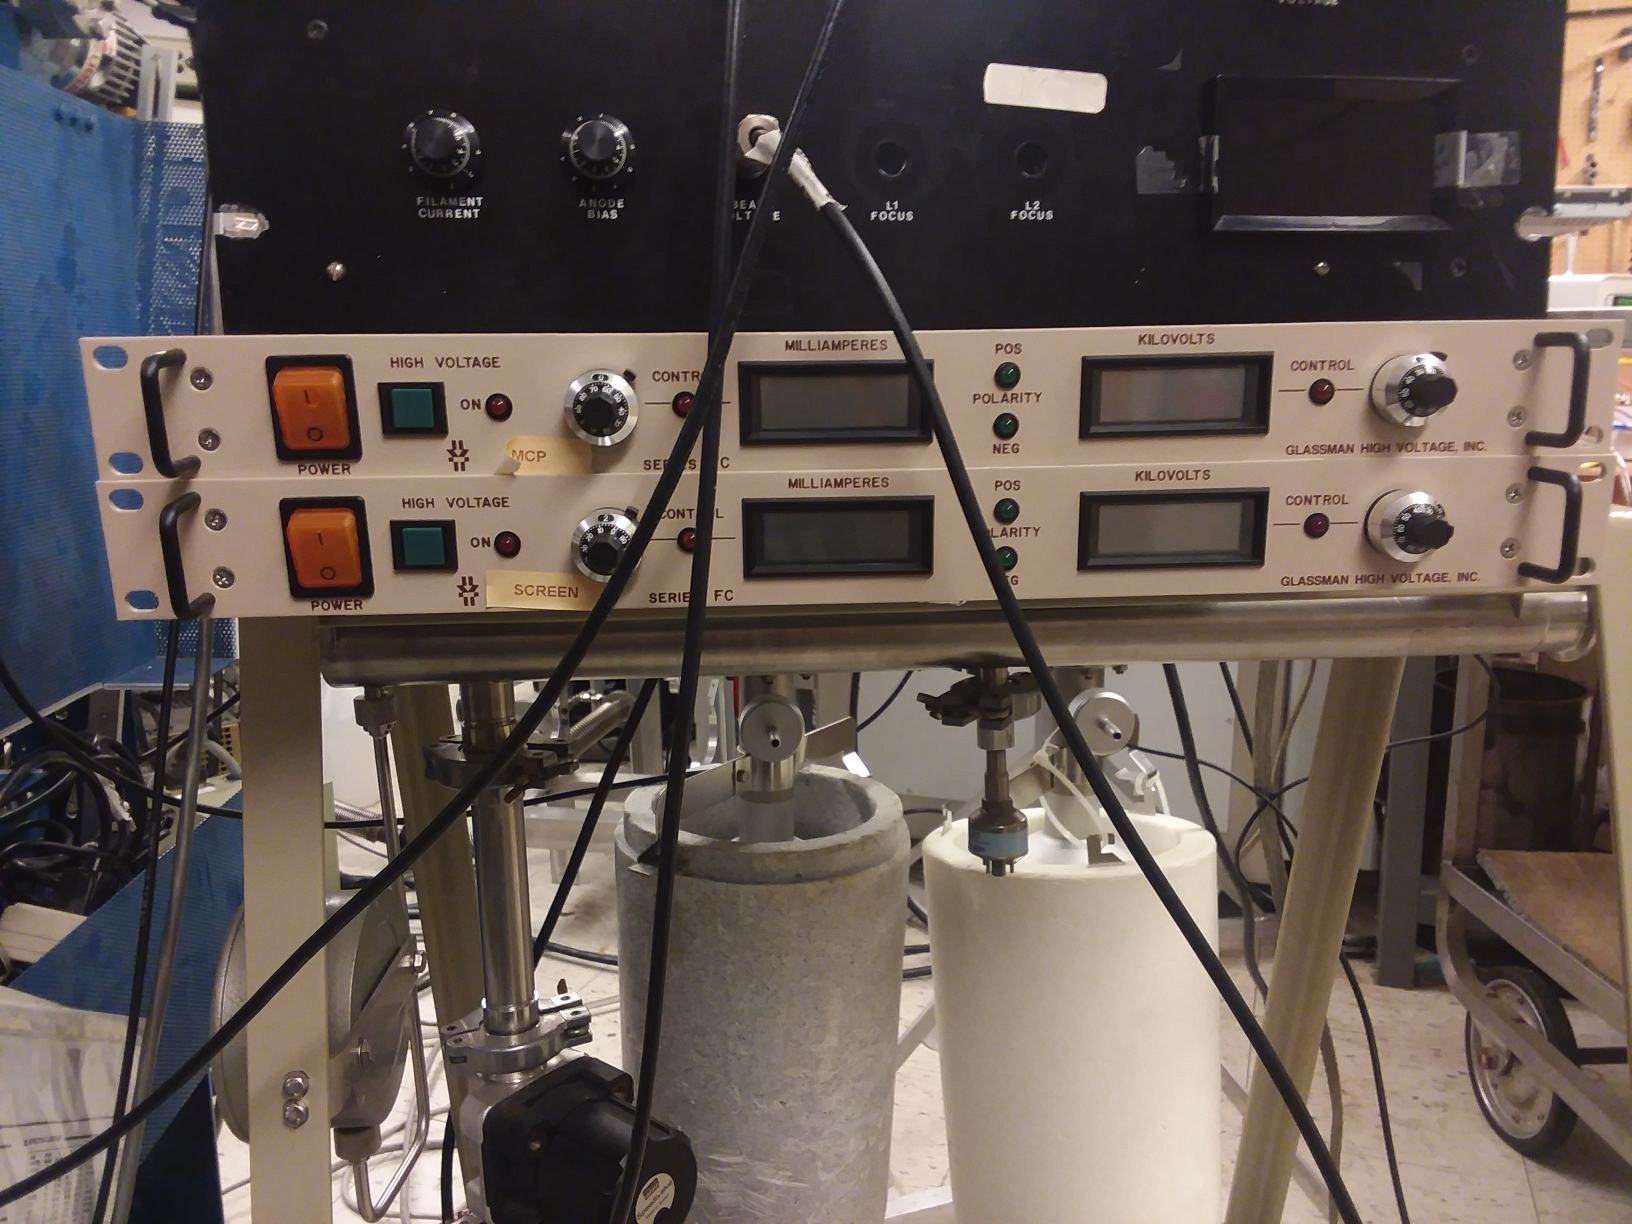
\includegraphics[width=0.75\textwidth]{beamvolt_n_lens_supply.png}
\caption{This displays the external power supplies used in conjunction with the sputter ion gun power supply. }
\label{SIGPSa}
\end{figure}

%%%%%%%%%%%%%%%%%%%%%%%%%%%%%%
\subsubsection{Sputter Gun (SG) connections }
%%%%%%%%%%%%%%%%%%%%%%%%%%%%%%
There are few key connections to get the sputter gun to work: Lens $1$ and $2$, anode, filament common (COM), and filament $1$ and $2$. These are displayed in figure \ref{sputtgun}. The breakdown of the different letters corresponds to the following:

\begin{enumerate}
	\item  Pin group $1$:
       \begin{enumerate}
                 \item empty (/not connected to anything) 
                 \item  empty
                 \item filament $\# 1$ 
                 \item filament common 
       \end{enumerate}
	\item Pin group $2$:
       \begin{enumerate}
                 \item empty 
                 \item  empty
                 \item empty 
                 \item empty 
       \end{enumerate}
	\item  Pin group $3$:
       \begin{enumerate}
                 \item empty 
                 \item  empty
                 \item empty 
                 \item empty 
       \end{enumerate}
           \item  Pin group $4$: 
      \begin{enumerate}
                 \item Lens $1$ focus 
                 \item  Lens $2$ focus
                 \item filament $\# 2$ 
                 \item Anode
       \end{enumerate}
\end{enumerate}

\begin{figure}[H]
\includegraphics[width=0.75\textwidth]{sputter_gun_connections.png}
\caption{This shows the connections to the sputter gun. }
\label{sputtgun}
\end{figure}

PRJ and DM tested the connections to the sputter gun Feb $3rd, \ 2020$. Lens $1$ seemed to have something off (inside), filament $\# 1$ was not connected, and Anode, Lens $2$, filament common, and filament $\# 2$ was connected. $1$ D and $1$ B seemed to be shorted somehow or filament $\# 1$ could be burnt out but the fact that $1 D$ and $1 B$ are connected is suspicious. In order to find out one will need to turn to troubleshooting section.(Taking the actual sputter gun apart.)


\begin{figure}[H]
\includegraphics[width=0.75\textwidth]{real_gun_connections.png}
\caption{This shows what the actual connections to the sputter gun look like. }
\label{realgun}
\end{figure}


In order to utilize the sputter gun one must have a gas to sputter with. In our lab we use Argon. Its relatively cheap and easy to make ionized gas to sputter a metallic surface with. The important thing is how much gas we send through the sputter gun so we don't flood the entire main chamber with Argon which could destroy sensitive electronics and pumps connected to our ultra high vacuum. The procedure for using this gas knob will be depicted in a later section. The gas knob is displayed in figure  \ref{gasknob}. Then this is connected to to the gas line port of the sputter gun as shown in figure \ref{sputtgun}.

\begin{figure}[H]
\includegraphics[width=0.75\textwidth]{gas_knob.png}
\caption{This displays the gas knob which controls the flow of the noble gas through the sputter gun. }
\label{gasknob}
\end{figure}

%---------------------------------------------------------------------------------------------
%----------------------------Connections-----------------------------------------
%----------------------------------------------------------------


%------------------------------------------------------------------
%---------------------------Operating the SIGPS----------------------------
%-------------------------------------------------------------------------------------------
\subsection{Operating the Sputter Gun}
At this point we will assume you read the connections section and have the sputter gun power supply and external power supplies connected to the sputter gun. We also assume that you connected the gas source to the sputter gun. Assuming that you turned all of the knobs back to zero. Make sure if you have any ion gauges on that you turned them off as well as closing the gate valve for any ion pumps you have running in your chamber. (Ion pumps do not like Argon ions/atoms...)

First turn on the external power supplies, click on the green button (high voltage). This allows the external supplies to be controlled for high voltages. Then turn on the SIGPS. Have a Digital multimeter with a high voltage probe ready to test the output as the display acts up on the SIGPS.

{\boxed:  You will want to connect the DMM to the anode to ensure what voltage is coming out of your system. (I might attach some wires for checking these more easily with the current set up.)  }

Now let's orient ourselves to the sputter guns gas knob. $0 \ 0 $ is the intial location of the knob when the sputter gun gas flow is closed by turning the knob all the way clockwise (to the right) and aligns with the same label below the knob. Depending on baking this sticker may need to be replaced to have the correct starting location. Meanwhile the $1 / 2 $ sticker represents a half turn on the knob. These are displayed in figure \ref{gassticker}. 

\begin{figure}[H]
\includegraphics[width=0.75\textwidth]{sputter_gas_knob.png}
\caption{This displays the gas knob with the full turn and the half turn stickers. This knob controls the flow of the noble gas through the sputter gun. }
\label{gassticker}
\end{figure}


Next we will want to add Argon to the system. When we tested this on Feb $20th, \ 2020$ the pressure in the Main Chamber was $2.6 \ e \ -9$ torr prior to releasing Argon. Turning the valve for $4$ rotations we saw a rise in pressure to $1.0 \ e \ -7$ torr, and turning the valve for $4.5$ rotations we saw a rise in pressure to $3.5 \ e \ -6$. We tested the sputter gun at $4.5$ turns. 

 Set the lens voltage to $300$ V and the beam voltage to $500$ V. Then measure the current from your sample. After you are done with your test, close the gas knob, then turn off the SIGPS and the external power supplies. If you are using an ion pump on your system after you have closed the gas line you may open the gate valve back up that contains your ion pump to pump on the main chamber.

%---------------------------------------------------------------------------------------------
%----------------------------Operating the SIGPS-----------------------------------------
%----------------------------------------------------------------
%------------------------------------------------------------------
%---------------------------Trouble Shooting----------------------------
%-------------------------------------------------------------------------------------------
\subsection{Troubleshooting}
This is where we talk about taking it apart and trouble shooting each device inside the Sputter Ion Gun Power Supply...testing the SIGPS on the bench with the filament, high voltage probe, etc.

%---------------------------------------------------------------------------------------------
%----------------------------Trouble Shooting-----------------------------------------
%----------------------------------------------------------------

\subsection{Acknowledgements}
Thank you Patrick Johnson and Dr. Sosolik for helping me test this sputter gun, troubleshoot parts, providing historical resources for fixes, and your advice along the way.

\twocolumn
\newpage

%----------------------------------------------------------------------------------
%--------------Acronyms ---------------------------------
%----------------------------------------------
\appendix
\chapter{Acronyms}
\textbf{HVPS} - High Voltage Power Supply
\\
\textbf{SIGPS} - Sputter Ion Gun Power Supply
\\
\textbf{SG} - Sputter Gun

%\newpage
%chicago
%\bibliographystyle{plainnat}
%\bibliography{words}


\end{document}

